\section{Theories of new physics}
\label{sec:BSMintro}

The standard model of particle physics has been very successful in describing observations. 
However, as explained in the previous section, this framework leaves several unanswered fundamental questions.
Many extensions to the standard model have been proposed that attempt to address the open issues and to achieve a more fundamental theory
that could explain the entirety of current phenomena.
These new theoretical developments are referred to as theories \textit{beyond standard model} (BSM).
In this section, three specific BSM scenarios are reviewed, which are of particular interest because of their highly predictive features.
Specifically, with the aim of addressing the hierarchy problem of the SM, they predict the existence of new resonances with masses in the TeV range,
which can be produced at hadron colliders.
Furthermore, since the new resonances can decay into pairs of well-known standard model particles, their existence and properties can be directly probed by collider experiments.
In particular, the decay modes into a pair of electroweak bosons \PW, \PZ or \PH, can provide striking signatures, as new techniques have been developed by the experiments to efficiently reconstruct the decay and mass of the bosons in the final state.

%%%%%%%%%%%%%%%%%%%%%%%%%%%%%%%%%%%%%%%%%%%%
\subsection{Warped extra dimensions}\label{subsec:graviton}
%%%%%%%%%%%%%%%%%%%%%%%%%%%%%%%%%%%%%%%%%%%%

A class of theories beyond the standard model postulates the existence of new compactified spatial dimensions.
They attempt to explain the apparent weakness of the gravitational force by assuming that SM particles are confined in a (3+1)-dimensional hypersurface called a \textit{3-brane},
as opposed to the gravitational force which is allowed to propagate in a (4+n)-dimensional \textit{bulk}.
In this scenario, the strength of the gravitational force is diluted in the extra dimensions (thereby weakening our perception of the gravitational force), while the other fundamental forces would not.

The basic idea comes from the so-called \textit{large extra dimensions} scenario proposed by Arkani-Hamed, Dimopoulos and Dvali (ADD model)~\cite{ArkaniHamed:1998rs}.
If spacetime has 4+$n$ dimensions, then the effective 4-dimensional (reduced) Planck scale, $\bMPl = \MPl/\sqrt{8\pi}$,
is determined by the fundamental (4+$n$)-dimensional Planck scale, $M_*$, and the geometry of the extra dimensions:

\begin{equation}\label{eqn:WED_1}
\bMPl^2 = V_nM^{n+2}_* \simeq R^nM^{n+2}_*,
\end{equation}

\noindent where $V_n$ is the volume of the $n$-dimensional compactified space and $R$ its radius.
The hierarchy problem is thus eluded if $M_* \sim 1\TeV$, which turns into a condition on the size $R$ of the extra dimensions.
Assuming $n = 1$, one can solve Eq.~\ref{eqn:WED_1} and obtain $R \sim 10^8\unit{m}$.
This is a scale of the order of the Earth-Sun distance, over which we know that the $1/r^2$ Newton's law of gravitational attraction works very well. Thus, $n = 1$ is excluded.
For $n = 2$, one obtains $R \sim 100\mum$ or $R^{-1} \sim 10^{-4}$\unit{eV}, which is close to the limit of current table top experimental searches for deviations from the Newton's law~\cite{Hoyle:2004cw}. 

The purpose of this model was to eliminate the hierarchy problem, i.e. to remove the large ratio between the weak scale $v$ and the true fundamental scale \bMPl, hence the requirement $M_* \sim 1\TeV$.
However, it introduces a new hierarchy, namely that between the compactification scale $\mu_c = 1/R$ and $v$.
Thus, the ADD really only trades one large ratio for another and does not really eliminate the hierarchy problem.
An alternative solution, represented by the so-called \textit{warped extra dimensions} (WED) scenario, has been proposed by Randall and Sundrum (RS)~\cite{Randall:1999ee}.

\begin{wrapfigure}{R}{0.4\textwidth}
 \centering
 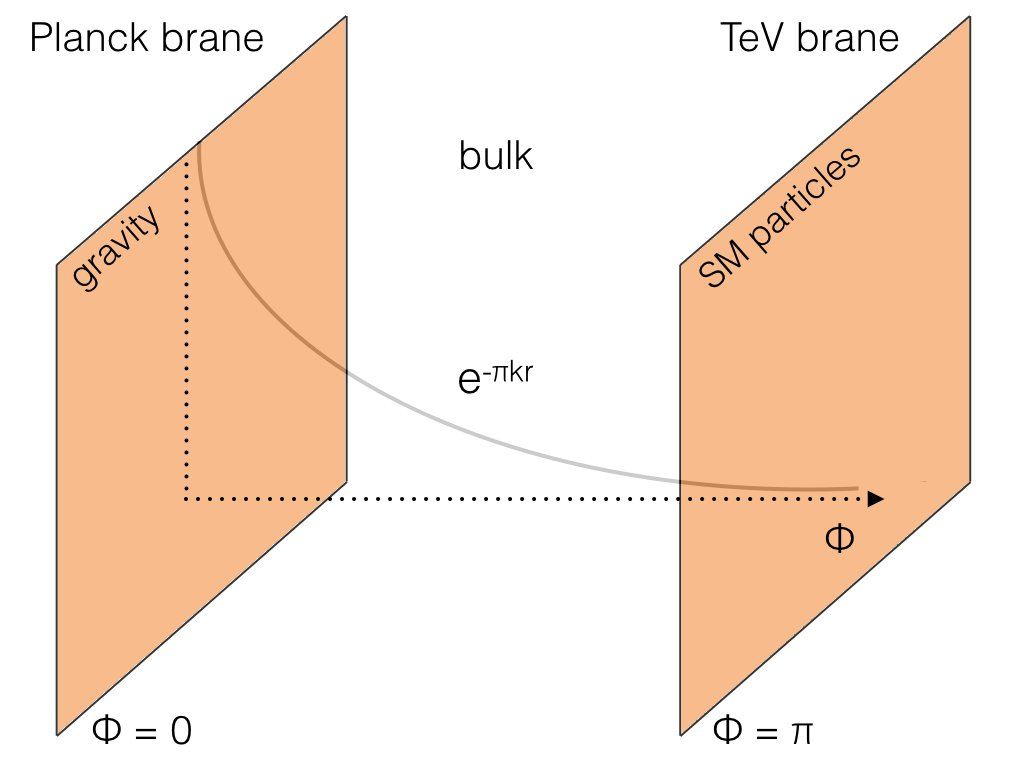
\includegraphics[width=0.35\textwidth]{\chtwo/RS1model.png}
 \caption{Setup of the five dimensions in the RS1 model. The \textit{Planck} and \textit{TeV} branes are the 4-dimensional boundaries of the extra dimension $\phi$ compactified in an interval $[0,\pi]$.}
 \label{fig:WED}
\end{wrapfigure}

The basic RS model, referred to as RS1, assumes the existence of only one extra dimension with size $r_c$. This fifth, extra dimension is labelled by the coordinate $\phi \in [-\pi,\pi]$,
such that it can be described by a line segment between two 4-dimensional branes (or 3-branes), known as the \textit{Planck} and \textit{TeV} brane, located, respectively,
at the $\phi = 0$ and $\phi = \pi$ boundary of the fifth dimension (Fig.~\ref{fig:WED}).
In the simplest version of the RS model, it is assumed, as in the ADD case, that the SM fields exist on the \textit{TeV} brane, while the gravitational force lives everywhere.
The \textit{Planck} brane is where the gravitational force is relatively strong.
The classical action describing the above setup is given by the sum of the gravitational action in the bulk, $\mathcal{S}_{gravity}$, and on the two branes, $\mathcal{S}_{TeV}$ and $\mathcal{S}_{Planck}$,

\begin{equation}\label{eqn:WED_2}
\begin{gathered}
\mathcal{S} = \mathcal{S}_{gravity} + \mathcal{S}_{TeV} + \mathcal{S}_{Planck}, \\
\mathcal{S}_{gravity} = \int d^4x \int_{-\pi}^{+\pi} d\phi\sqrt{-G}(-\Lambda+2M^3_*R), \\
\mathcal{S}_{TeV} = \int d^4x\sqrt{-G(x^\mu,\phi=\pi)}\Lambda, \\
\mathcal{S}_{Planck} = \int d^4x\sqrt{-G(x^\mu,\phi=0)}\Lambda.
\end{gathered}
\end{equation}

In the above equation, $G$ is the 5-dimensional metric $G_{\mu\nu}$, $\Lambda$ a cosmological constant, and $R$ the 5-dimensional Ricci tensor.
By requiring a solution of the 5-dimensional Einstein's equation for the above action that respects the 4-dimensional Poincar\'{e} invariance in the $x^\mu$ coordinates,
one finds that the 5-dimensional metric must take the form 

\begin{equation}\label{eqn:WED_3}
ds^2 = e^{-2\sigma(\phi)} \eta_{\mu\nu}dx^\mu dx^\nu + r^2_cd\phi,
\end{equation}

\noindent where $\eta_{\mu\nu} = \mathrm{diag}(1,-1,-1,-1)$ is the usual Minkowski metric and $\sigma(\phi)$ is some a-priori unknown function.
This type of geometry is called ``non-factorizable'', because the metric of the 4-dimensional subspace is $\phi$-dependent.
Solving the 5-dimensional Einstein's equations provides a unique solution for $\sigma(\phi)$:

\begin{equation}\label{eqn:WED_4}
\sigma(\phi) = \sqrt{\frac{-\Lambda}{24M^3_*}} \equiv r_c|\phi|k,
\end{equation}

\noindent where $k$ is referred to as the \textit{curvature factor}.
By plugging the solution back into the original action and integrating over the extra dimension $\phi$, one finds that the 4-dimensional Planck mass is given by

\begin{equation}\label{eqn:WED_5}
\bMPl^2 = \frac{M^3_*}{k}(1 - e^{-2\pi kr_c}).
\end{equation}

%\noindent where the term $e^{-2\pi kr_c}$ is usually called the \textit{warp factor}.
It is assumed that $k \sim M_* \sim \bMPl$ in order to avoid producing a strong hierarchical difference between the mass scales of the theory.
However, the electroweak energy scale $v$ or any physical mass $m$ in the \textit{TeV} brane is exponentially suppressed compared to the 5-dimensional energy $v_0$ or mass $m_0$:

\begin{equation}\label{eqn:WED_6}
m = e^{-\pi kr_c}m_0 \, , \qquad\qquad v = e^{-\pi kr_c}v_0.
\end{equation}

This means that by taking $v_0$ of the order of the 5-dimensional fundamental mass scale $M_*$, the separation between the Planck and electroweak scales
is produced by the metric when $kr_c \sim 11$ (small hierarchy). Such a factor indeed would already suppress a parameter with value of order $10^{18}\GeV$ to only 1\TeV.
The hierarchy is thus naturally established by the warp factor $e^{-\pi kr_c}$.
This Planck-electroweak hierarchy explanation is the most celebrated achievement of WED scenarios.

A distinctive novel feature of the RS scenario is the existence of a so-called tower of Kaluza--Klein (KK) excitations of a spin-2 field, the KK graviton, arising from tensor fluctuations 
around the 4-dimensional part of the metric. Scalar fluctuations around the fifth extra dimension give rise to a spin-0 field called the \textit{radion}.
Massive graviton excitations appear, with 4-dimensional effective masses given by

\begin{equation}\label{eqn:WED_7}
m_G^{(n)} = kx_ne^{-\pi kr_c},
\end{equation}

\noindent where $x_n$ is the $n$-th root of the Bessel function $J_1$. These masses are of order of a TeV, so that Kaluza-Klein gravitons can be detected as massive resonances in collider experiments. 
The zero-mode of the graviton field corresponds to the mediator of the gravitational interaction, and its wave function is highly peaked at $\phi = 0$. The gravitational force is thus localized on the \textit{Planck} brane, while on the \textit{TeV} brane we feel only the tail of the graviton wave-function. %So in the RS model the reason of the weakness of gravity is that it is localized far away from where we live.

The coupling of an excited graviton to matter is described by the Lagrangian

\begin{equation}\label{eqn:WED_8}
\mathcal{L} = - \frac{1}{\Lambda_\pi}T^{\mu\nu}\sum_{n>0}h^{(n)}_{\mu\nu},
\end{equation}

\noindent where $T^{\mu\nu}$ is the energy-momentum tensor of the matter field, $h^{(n)}_{\mu\nu}$ is the $n$-th excitation of the graviton,
and $\Lambda_\pi = \bMPl e^{-\pi kr_c}$ is of order of a TeV.
It is interesting to note that this model has only two free parameters: the mass of the first (lightest) KK-graviton excitation, $m_1$, and the ratio $\tilde{k} \equiv  k/\bMPl$, which controls the widths of the new resonances:

\begin{equation}\label{eqn:WED_9}
\Gamma_n = \rho m_n x^2_n\tilde{k}^2,
\end{equation}

\noindent where $\rho$ is a constant depending on the number of open decay channels.
The RS model in its simplest form is thus highly predictive.\\

In the original RS1 model the SM matter is localized on the \textit{TeV} brane, as the Higgs field.
A well-motivated extension of the original RS1 model explores an alternative scenario, in which 
SM fields propagate in the warped bulk, except for the Higgs field which is required on the \textit{TeV} brane to avoid a large hierarchy.
This extension is referred thereafter as the \textit{bulk scenario}~\cite{Agashe:2007zd,Fitzpatrick:2007qr}.
Similarly to the KK-graviton excitations, in the bulk scenario a KK expansion is applied to each SM field.
The zero-mode of each KK tower represents the correspondent SM particle.
The first and second generation fermions are localized near the \textit{Planck} brane, leading to the the small Yukawa couplings to the Higgs field which is localized on the \textit{TeV} brane.
Similarly, the top quark can be localized near the \textit{TeV} brane to account for its large Yukawa coupling.
In the original RS1 scenario all the particles are localized on the \textit{TeV} brane, therefore the strength of the couplings between KK-graviton and SM particles are democratic. 
As a consequence, the RS gravitons are produced via both \qqbar annihilation and gluon fusion processes.
In the bulk scenario, couplings of KK gravitons to light fermions are highly suppressed since, as mentioned above, KK gravitons are localized near the \textit{TeV} brane, whereas light fermions are localized near the \textit{Planck} brane. As a result, \qqbar annihilation at hadron collider for KK graviton production is negligible in this case.
In contrast, SM gluons have a flat localization in the bulk, so that the coupling of gluons to KK gravitons and hence KK graviton production via gluon fusion is dominant.
Furthermore, decays of KK graviton into top quarks and Higgs bosons are enhanced due to being localized near the \textit{TeV} brane, resulting in couplings to KK gravitons (which are also localized there) being only $\sim\TeV$-suppressed just like in the original RS1 model (Eq.~\ref{eqn:WED_8}).
Another crucial point of the bulk scenario is that before symmetry-breaking, the \PW and \PZ gauge bosons start out with flat localization in the bulk. %and the Higgs starts out with a delta function wave-function on the brane.
However, after symmetry-breaking, the gauge bosons absorb the Higgs degrees of freedom, and their wave functions are still mostly flat in the bulk but fall sharply near the brane.
Thus, in the bulk scenario, branching fractions for decays into a pair of vector bosons are the same level as those for decays into Higgs bosons or top quarks.
The branching fractions for the different decay modes of the graviton in both the bulk and RS1 scenarios are shown in Fig.~\ref{fig:GrBR} as a function of the graviton mass.
It can also be shown that in RS1 scenario the graviton decays preferentially to transversely-polarized vector bosons, whereas in the bulk scenario it decays preferentially to longitudinally-polarized modes, making those two benchmarks an excellent framework for studying the sensitivity of the vector boson identification techniques used at the collider experiments to the polarization (Chapter~\ref{ch:vtagging}).

\begin{figure}[!htb]
\centering
\subfigure[]{\label{fig:GrBR_a}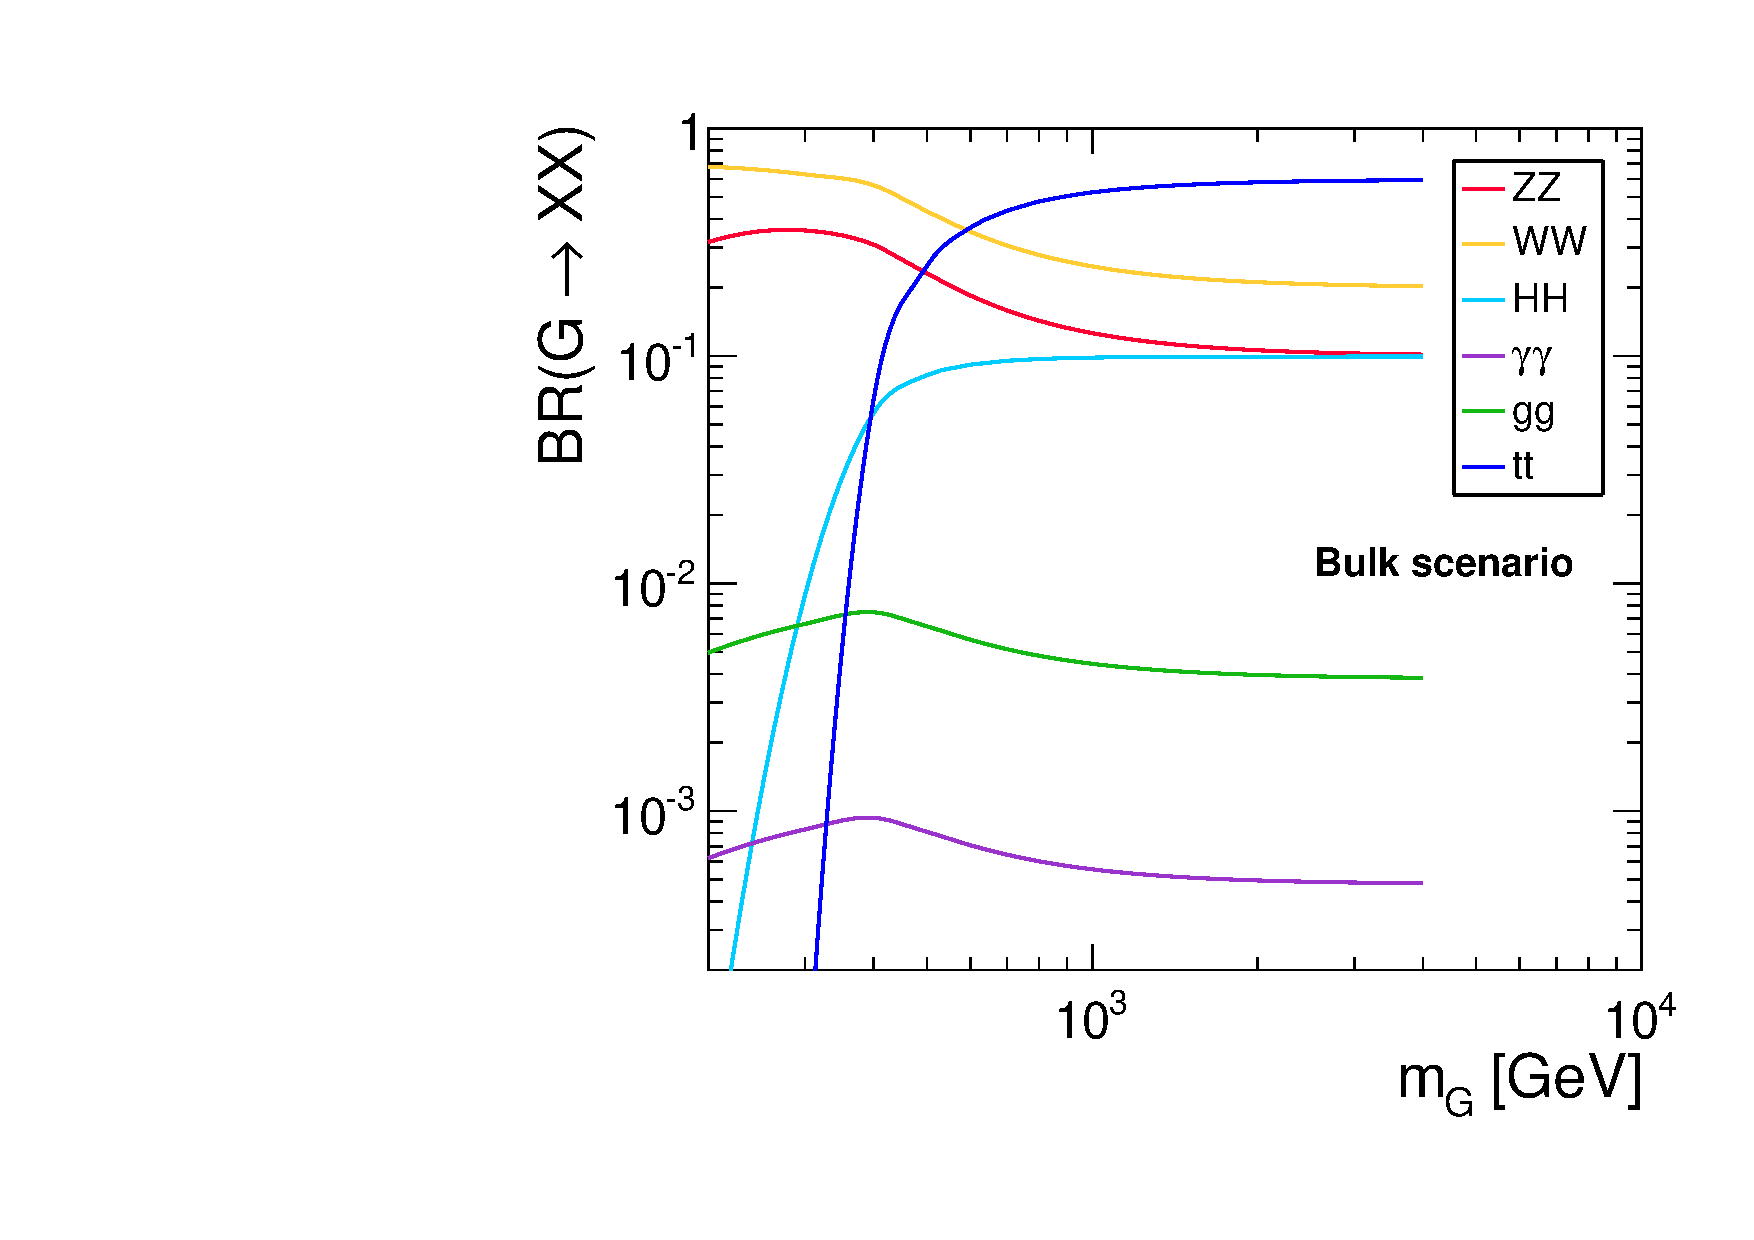
\includegraphics[width=0.45\textwidth]{\chtwo/brs-bulkg.pdf}}
\subfigure[]{\label{fig:GrBR_b}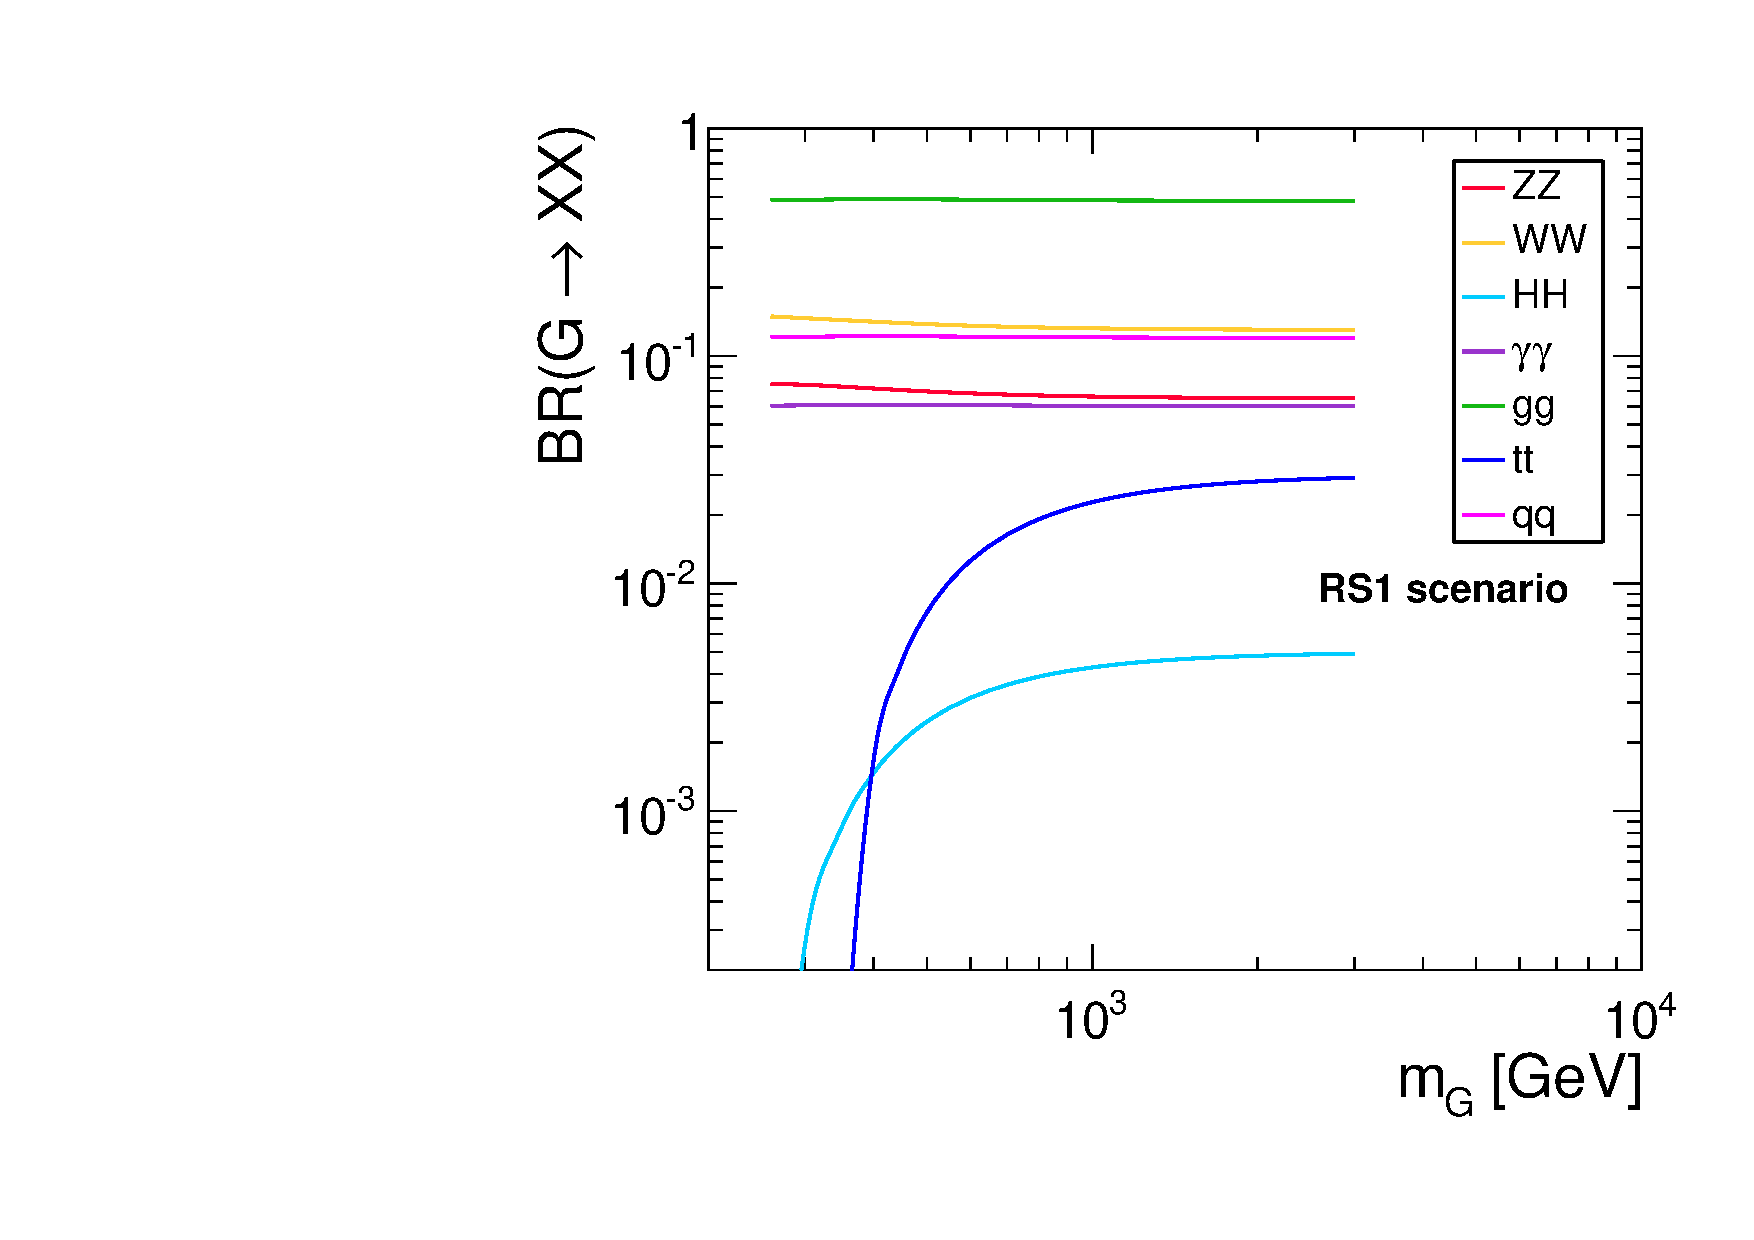
\includegraphics[width=0.45\textwidth]{\chtwo/brs-rs1.pdf}}
\caption{Branching fractions for the different decay modes of the graviton in the (a) bulk and (b) RS1 scenarios, as a function of the graviton mass.}
\label{fig:GrBR}
\end{figure}

%%%%%%%%%%%%%%%%%%%%%%%%%%%%%%%%%%%%%%%%%%%%
\subsection{Compositeness}\label{subsec:composite}
%%%%%%%%%%%%%%%%%%%%%%%%%%%%%%%%%%%%%%%%%%%%

One of the approaches to the hierarchy problem compatible with observations is based on the assumption that the Higgs boson is a composite particle, a bound state of more fundamental constituents held together by a new strong force.
In composite Higgs models~\cite{Composite0,Composite1,Composite2}, $\Lambda$ is the energy scale where the composite nature of the Higgs boson becomes important, which roughly coincides with the confinement scale of the new strong interaction. Thus, the solution to the hierarchy problem is that there is no elementary scalar, and beyond $\Lambda$ an experiment becomes sensitive to the underlying ``partons'' that compose the Higgs boson. 
However, precision electroweak data rule out new strong interactions at scales below about 10\TeV.
One key question is therefore the lightness of the Higgs boson with respect to such a scale.

By comparing with the QCD sector, one observes that the strong coupling scale is $\Lambda_\mathrm{QCD} \sim \mathcal{O}(300\MeV)$, whereas most bound states, such as the $\rho$ meson and proton, are at least as heavy as this.
However, a counter-example in QCD is given by the existence of the pions, which are all lighter than $\Lambda_\mathrm{QCD}$, although only by a $\mathcal{O}(1)$ factor.
The reason for the pions to be appreciably lighter than the other QCD bound states is found in the chiral perturbation theory. 
In fact, the pions represent the Goldstone bosons of the spontaneously broken $SU(2)_L \times SU(2)_R$ flavor symmetry coming from chiral rotations of the up and down quarks. 
The spontaneous symmetry breaking of the flavor symmetry into the vectorial isospin subgroup $SU(2)_V$, is induced by a non-perturbative QCD vacuum state, characterized by a non-vanishing quark condensate $\langle \bar{q}^a_L q^b_R \rangle \sim \delta^{ab}\Lambda^3_\mathrm{QCD}$.
However, because of the non-vanishing and differing masses of the quarks, the $SU(2)_L \times SU(2)_R$ is only an approximate symmetry, and therefore the pions are not massless, but have small masses, so that they are \textit{pseudo-Goldstone bosons}.

In composite Higgs models, a similar structure is assumed, where the Higgs is a pseudo-Goldstone boson of some symmetry with strong coupling scale $\Lambda \approx 4\pi f$,
where $f$ is the scale at which the symmetry is spontaneously broken.
The main idea is that the Higgs-boson mass parameter is protected against quadratic quantum corrections up to the compositeness scale because it is a pseudo-Goldstone boson. 
Above the scale of compositeness, it is simply not an elementary scalar.
Furthermore, the pseudo-Goldstone nature of the Higgs is an explanation for why the Higgs-boson mass is so much lighter than the other bound states in the strongly coupled sector.

Such models start with a large global symmetry group $G$, analogous to the ``large'' $SU(2)_L \times SU(2)_R$ global symmetry of low energy QCD.
The strong dynamics spontaneously breaks $G$ to a subgroup $H$, similarly to the QCD chiral symmetry breaking $SU(2)_L \times SU(2)_R \to SU(2)_V$.
In particular, for a minimal composite Higgs model $G = SO(5) \to H = SO(4)$.
The SM electroweak group $SU(2)_L \times U(1)_Y$ is a subgroup of $H$, thus introducing a preferred orientation in the coset space SO(5)/SO(4) with respect to the global SO(4).
In this way, the electroweak scale $v$ is distinct from the $G \to H$ symmetry breaking scale $f$. The parameter $\xi = (v/f)^2$ is introduced to characterize this separation of scales and to quantify the degree of vacuum misalignment.
In a theory with little hierarchy $\xi \sim 1$, while a small amount of fine-tuning can give rise to $\xi \ll 1$. In particular, compatibility with the constraints coming from electroweak precision tests and Higgs coupling measurements generically implies $\xi \lesssim 0.2$. This bound places the scale $f$ at about 1\TeV, resulting in a strong coupling scale $\Lambda \approx 4\pi f \sim 10\TeV$.
Such large value results in a large one-loop contribution to the Higgs-boson mass parameter (Eq.~\ref{eqn:HiggsCorr}), so that a generic composite Higgs setup still requires some tuning between the $v$ and $f$ scales.
One way to generate a ``little hierarchy'' is through the mechanism of \textit{collective symmetry breaking} as in \textit{little Higgs} (LH) scenarios~\cite{Han:2003wu,Perelstein:2005ka,Schmaltz:2005ky,Arkani:2002LH,Burdman:2002ns}, which is now a key ingredient in composite Higgs models.
The main idea of this approach is that one can separate the scales $v$ and $f$ by introducing new particles, which cancel the quadratic divergences at one-loop order. 
In particular, the quadratic divergence induced by the SM gauge boson loops are canceled by the quadratic divergence induced by heavy gauge bosons at one loop level.
Heavy fermionic states are also introduced, which couple to the Higgs field such that the one-loop quadratic divergence induced by the top-quark Yukawa coupling to the Higgs boson is canceled.
Furthermore, extra Higgs fields exist as the Goldstone boson multiplets from the global symmetry breaking.
%In Little Higgs models, instead of a simple global group $G$ a direct product of two (or more) groups $G_1 \times G_2 \times \dotsc$ is considered so that its breaking has a collective nature.
%The models then contain additional gauge bosons at the TeV scale that produce the necessary cancellations to the one-loop quadratic divergence.
%It implies that any non-vanishing quantum contribution to the Higgs-boson mass parameter must necessarily be proportional to a product of all the gauge coupling constants corresponding to the different $G_i$ factors.
%Thus, setting any one of the coupling constants to zero must result in a vanishing contribution.
%The extended gauge group $G_1 \times G_2 \times \dotsc$ of the LH models is typically broken down to the SM $\mathrm{SU(2)_L \times U(1)_Y}$ at a scale $f$ by the same condensates that break $G \to H$.
%The models then contain additional gauge bosons at the TeV scale. In the mass eigenbasis, the vanishing of the one-loop quadratic divergence can be understood as a result of a cancellation between the SM bow tie diagrams and their counterparts involving the TeV-scale bosons. 
This is achieved by enlarging the simple global group $G$ and embedding two parallel global symmetries $G_1 \times G_2$, such that $G \supset G_1 \times G_2 = [SU(2)_1 \times U(1)_1] \times[SU(2)_2 \times U(1)_2]$.
A specific implementation, called the \textit{littlest Higgs}~\cite{Arkani:2002LH,Burdman:2002ns}, starts with the global symmetry $G$ = SU(5), which is spontaneously broken down at the scale $\Lambda$ to its subgroup $SO(5)$ via a vacuum expectation value of order $f$. At the same time, the gauge symmetry $[SU(2) \times U(1)]^2$ is also broken into $[SU(2)_L \times U(1)_Y]$, identified as the SM gauge group.
The global symmetry breaking leaves 14 massless Goldstone bosons, which become the longitudinal components of the $\mathrm{W}^{\prime\pm}$  and $\PZpr$ gauge bosons associated with the broken gauge groups, giving them masses of the order $f$:

\begin{equation}\label{eqn:LHvprimeMass}
M(\mathrm{W}^{\prime\pm}) \simeq M(\PZpr) = \frac{g}{\sin2\theta}f,
\end{equation}

\noindent where $\theta$ is given by the gauge couplings of the two broken $SU(2)$ groups: $\tan\theta = g_1/g_2$.
The partial decay widths are computed using the formalism of Feynman rules:

\begin{equation}
\begin{aligned}
\Gamma(\mathrm{W}^{\prime\pm} \to \ell\nu) & \simeq \Gamma(\PZpr \to \ell\ell) & = \frac{g^2\cot^2\theta}{96\pi}M\\
\Gamma(\mathrm{W}^{\prime\pm} \to \mathrm{q}\bar{\mathrm{q}}^\prime) & \simeq \Gamma(\PZpr \to \qqbar) & = \frac{g^2\cot^2\theta}{32\pi}M\\
\Gamma(\mathrm{W}^{\prime\pm} \to \PW\PH) & \simeq \Gamma(\PZpr \to \PZ\PH) & = \frac{g^2\cot^22\theta}{192\pi}M\\
\Gamma(\mathrm{W}^{\prime\pm} \to \PW\PZ) & \simeq \Gamma(\PZpr \to \PW\PW) & = \frac{g^2\cot^22\theta}{192\pi}M
\end{aligned} 
\end{equation}

\noindent where $M$ is the mass of the \PVpr triplet given by Eq.~\ref{eqn:LHvprimeMass}.
Summing over all the quark and lepton channels results in a total width

\begin{equation}\label{eqn:LHvprimeWidth}
\Gamma_\mathrm{tot} = \frac{g^2}{96\pi}(\cot^22\theta + 24\cot^2\theta)M.
\end{equation}

One can immediately observe that the fermionic decay modes dominate for $\cot\theta \geq 1/2$, while bosonic decay modes become significant only below this value.
However, since the \PVpr resonances are produced mainly via the Drell-Yan process $\qqbarpr \to \PVpr$, one should notice that the production cross section would be at the same time suppressed for the enhanced bosonic channels.
Thus, the interactions of the new predicted particles are described within these theories, and detailed predictions of their properties are made.
Furthermore, they provide distinct signatures that can be searched for at a hadron collider of sufficient energy.

%%%%%%%%%%%%%%%%%%%%%%%%%%%%%%%%%%%%%%%%%%%%
\subsection{Heavy vector triplet}\label{subsec:hvt}
%%%%%%%%%%%%%%%%%%%%%%%%%%%%%%%%%%%%%%%%%%%%

New heavy spin-1 resonances are predicted by several extensions of the standard model, such as the composite Higgs and little Higgs models described in the previous section.
A model-independent strategy has been proposed in Ref.~\cite{Pappadopulo:2014qza} to study these resonances, based on a simplified phenomenological Lagrangian, which reproduces a large class of explicit models.
The main reason for introducing a simplified model is that the experimental searches for new resonances are typically not sensitive to all the details and the free parameters of the chosen benchmark model, but only to those parameters or combinations of parameters that control the mass of the resonance and the interactions involved in its production and decay. Therefore one can employ a simplified description of the new phenomena, where only the relevant couplings and mass parameters are retained. In turn, the experimental results expressed in terms of the phenomenological parameters can be easily translated into the free parameters of any explicit model by computing the phenomenological/explicit parameter relations.\\

In this approach, a new real vector in the $\mathrm{SU(2)_L}$ representation is introduced in addition to the SM fields, describing one charged and one neutral heavy spin-1 particle (heavy vector triplet or HVT) with the charge eigenstate fields given by

\begin{equation}\label{eqn:HVT_1}
V^\pm_\mu = \frac{V^1_\mu \mp iV^2_\mu}{\sqrt{2}} \, \qquad\qquad V^0_\mu = V^3_\mu.
\end{equation}

The dynamics of the new vector is described by a simple phenomenological Lagrangian

\begin{equation}\label{eqn:HVT_2}
\begin{split}
\mathcal{L}_V = & -\frac{1}{4}\mathcal{D}_{[\mu}V^a_{\nu]}\mathcal{D}^{[\mu}V^{\nu]a} + \frac{m^2_V}{2}V^a_\mu V^{\mu a}\\
 & + ig_Vc_HV^a_\mu H^\dag\tau^a\overleftrightarrow{\mathcal{D}}^\mu H + \frac{g^2}{g_V}c_FV^a_\mu J^{\mu a}_F\\
 & + \mbox{extra terms}
 %& + \frac{g_V}{2}c_{VVV}\epsilon_{abc}V^a_\mu V^b_\nu\mathcal{D}^{[\mu}V^{\nu]c} + g^2_Vc_{VVHH}V^a_\mu V^{\mu a} H^\dag H - \frac{g}{2}c_{VVW}\epsilon_{abc}W^{\mu\nu a}V^b_\mu V^c_\nu,
 \end{split}
\end{equation}

\noindent where $g$ denotes the gauge coupling.
The first line of the above equation contains the kinetic and mass terms for the field $V$, plus trilinear and quadrilinear interactions with the vector bosons from the covariant derivatives.
The second line contains direct interactions of $V$ with the Higgs current in the first term, and with the SM left-handed fermionic currents $J^{\mu a}_F$ in the second term.
The Higgs current term with coefficient $c_H$ leads to vertices involving the physical Higgs field and the three unphysical Goldstone bosons.
Since the Goldstone bosons represent the longitudinally-polarized SM vector bosons \PW and \PZ, the parameter $c_H$ controls the interactions of $V$ with the SM vector bosons and with the Higgs boson, and in particular its decay modes into these electroweak particles.
Similarly, the parameter $c_F$ describes the direct interaction with fermions, which is responsible for both the resonance production via \qqbar annihilation and for its fermionic decays.
One observes that a universal coupling of the new field $V$ to fermions is assumed in Eq.~\ref{eqn:HVT_2} for simplicity, such that $c_F$ represents the couplings to leptons ($c_\ell$), light quarks ($c_q$) and the third quark family ($c_3$).
The third line of the equation contains new operators and free parameters, which however have a sub-leading effect on the phenomenology of interest for resonant searches, and
therefore to a first approximation they can be neglected.% and the phenomenology described entirely by the three parameters $c_H$, $c_F$, and the mass $m_V$ of the new states.

In the adopted simplified description, the free parameter $g_V$ represents the typical strength of $V$ interactions, while the dimensionless coefficient $c_H$ parametrizes the departure from the typical strength.
Such a parametrization is convenient because, although the coefficient $c_F$ is of order one in most of the explicit models, the parameter $c_H$ is of order one in the strongly-coupled scenario (e.g., composite Higgs models) but can be reduced in a weakly coupled case (e.g., extensions of the SM gauge group~\cite{PhysRevD.22.727,Altarelli}). The coefficients are never larger than one in all cases, whereas the coupling $g_V$ can vary over a large range in different scenarios, from $g_V \sim g \sim 1$ in the typical weakly-coupled case up to $g_V \sim 4$ in the strong limit. Therefore, it is more convenient to factor it out of the parametrization, although it is not a fundamental parameter of the model. For the purpose of presenting experimental results, the combinations $g_Vc_H$ and $g^2c_F/g_V$ that enter in the vertices are instead treated as fundamental parameters, as they control production and decay rates.

After electroweak symmetry breaking the heavy vector acquires mass and one finds that the charged and neutral $V$'s are practically degenerate ($M_\pm \simeq M_0 \simeq M_V$),
and therefore they are expected to have comparable production and decay rates at the hadron collider. The partial widths are as well immediately computed in this framework:

\begin{eqnarray}\label{eqn:HVT_3}
\Gamma_{V^\pm \rightarrow f\bar{f}^\prime} \simeq 2\Gamma_{V^0 \rightarrow f\bar{f}} & \simeq N_c[f] \left( \frac{g^2c_F}{g_V} \right)^2\frac{M_V}{48\pi}\nonumber \\
\Gamma_{V^\pm \rightarrow \PW\PZ} \simeq \Gamma_{V^0 \rightarrow \PW\PW} & \simeq \frac{g^2_Vc^2_HM_V}{192\pi}\\
\Gamma_{V^\pm \rightarrow \PW\PH} \simeq \Gamma_{V^0 \rightarrow \PZ\PH} & \simeq \frac{g^2_Vc^2_HM_V}{192\pi}\, , \nonumber
\end{eqnarray}

\noindent where $N_c[f]$ is the number of colors and is equal to three for the diquark and to 1 for the dilepton decays.
It can be observed that, through the partial width to qq, the parameter $c_F = c_q$ controls the Drell-Yan production rate.
The channels which are not reported in Eq.~\ref{eqn:HVT_3} are either forbidden, like $\PH\PH$ and $\gamma\gamma$ decays, or suppressed like the decays to transverse polarizations or to $\PW\gamma$.

Two exemplary benchmark models, called A and B, are studied in Ref.~\cite{Pappadopulo:2014qza}, which correspond to two explicit models describing heavy vectors, namely those in Refs.~\cite{PhysRevD.22.727} and~\cite{Composite1}, respectively. The $c_F$ and $c_H$ coefficients are fixed to specific values in these models, and the only free parameters are the resonance coupling $g_V$ and its mass $M_V$.
Moreover, since models A and B are inspired, respectively, by weakly-coupled extensions of the SM gauge group and strongly-coupled scenarios, i.e. composite Higgs models, the two benchmark models are considered in different regions of $g_V$, relatively small, $g_V \lesssim 3$, and relatively large, $g_V \gtrsim 3$, respectively. In particular, the branching fractions for the different decay modes of the neutral spin-1 resonance in models $\mathrm{A}_{g_V=1}$ and $\mathrm{B}_{g_V=3}$ are shown in Fig.~\ref{fig:hvtBR} as a function of the resonance mass. For these values of $g_V$, model A predicts comparable branching fractions for decay modes into fermions and bosons, as expected from Eq.~\ref{eqn:HVT_3}. In model B, on the contrary, $c_H$ is unsuppressed, and therefore the dominant branching fractions are into dibosons, whereas the fermionic decays are extremely suppressed.

\begin{figure}[!htb]
\centering
\subfigure[]{\label{fig:hvtBR_a}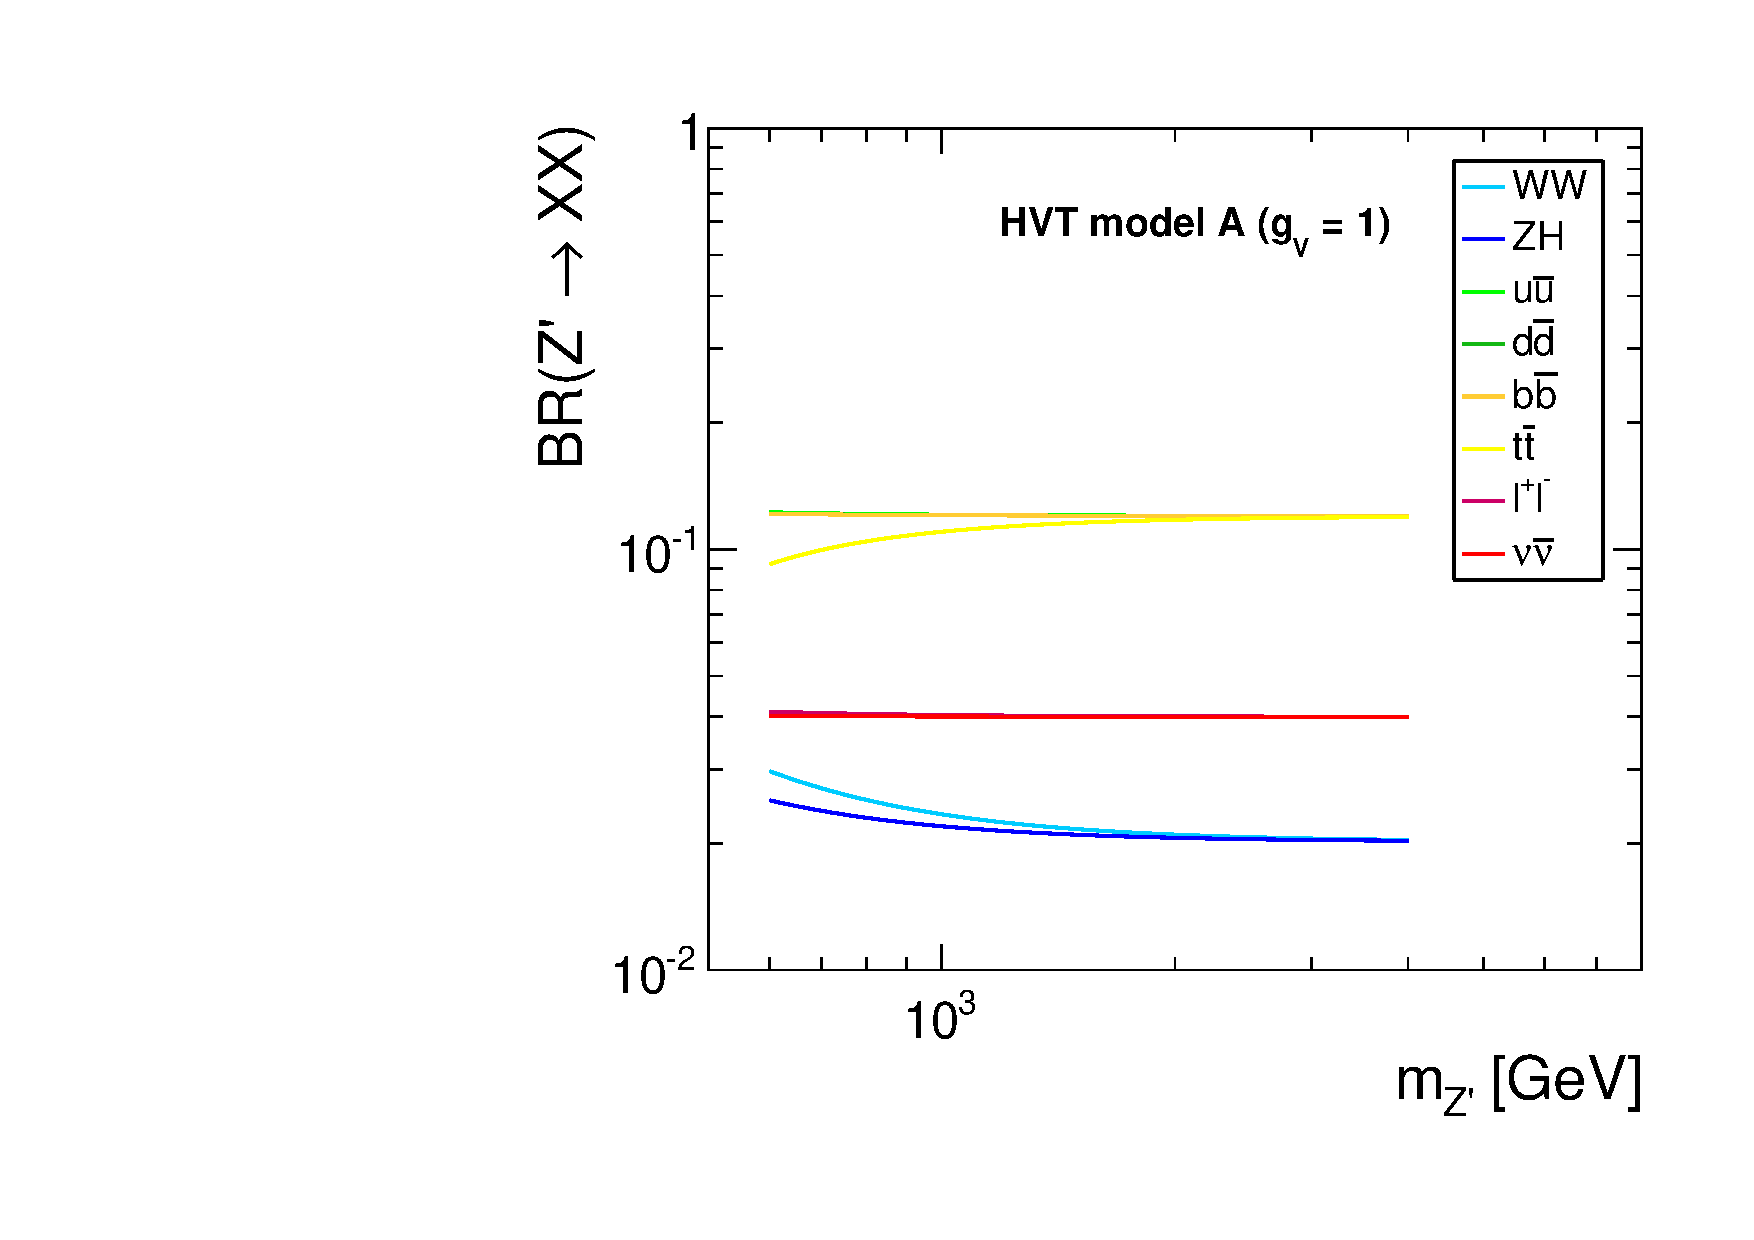
\includegraphics[width=0.45\textwidth]{\chtwo/brs-hvt-zprime-modelA.pdf}}
\subfigure[]{\label{fig:hvtBR_b}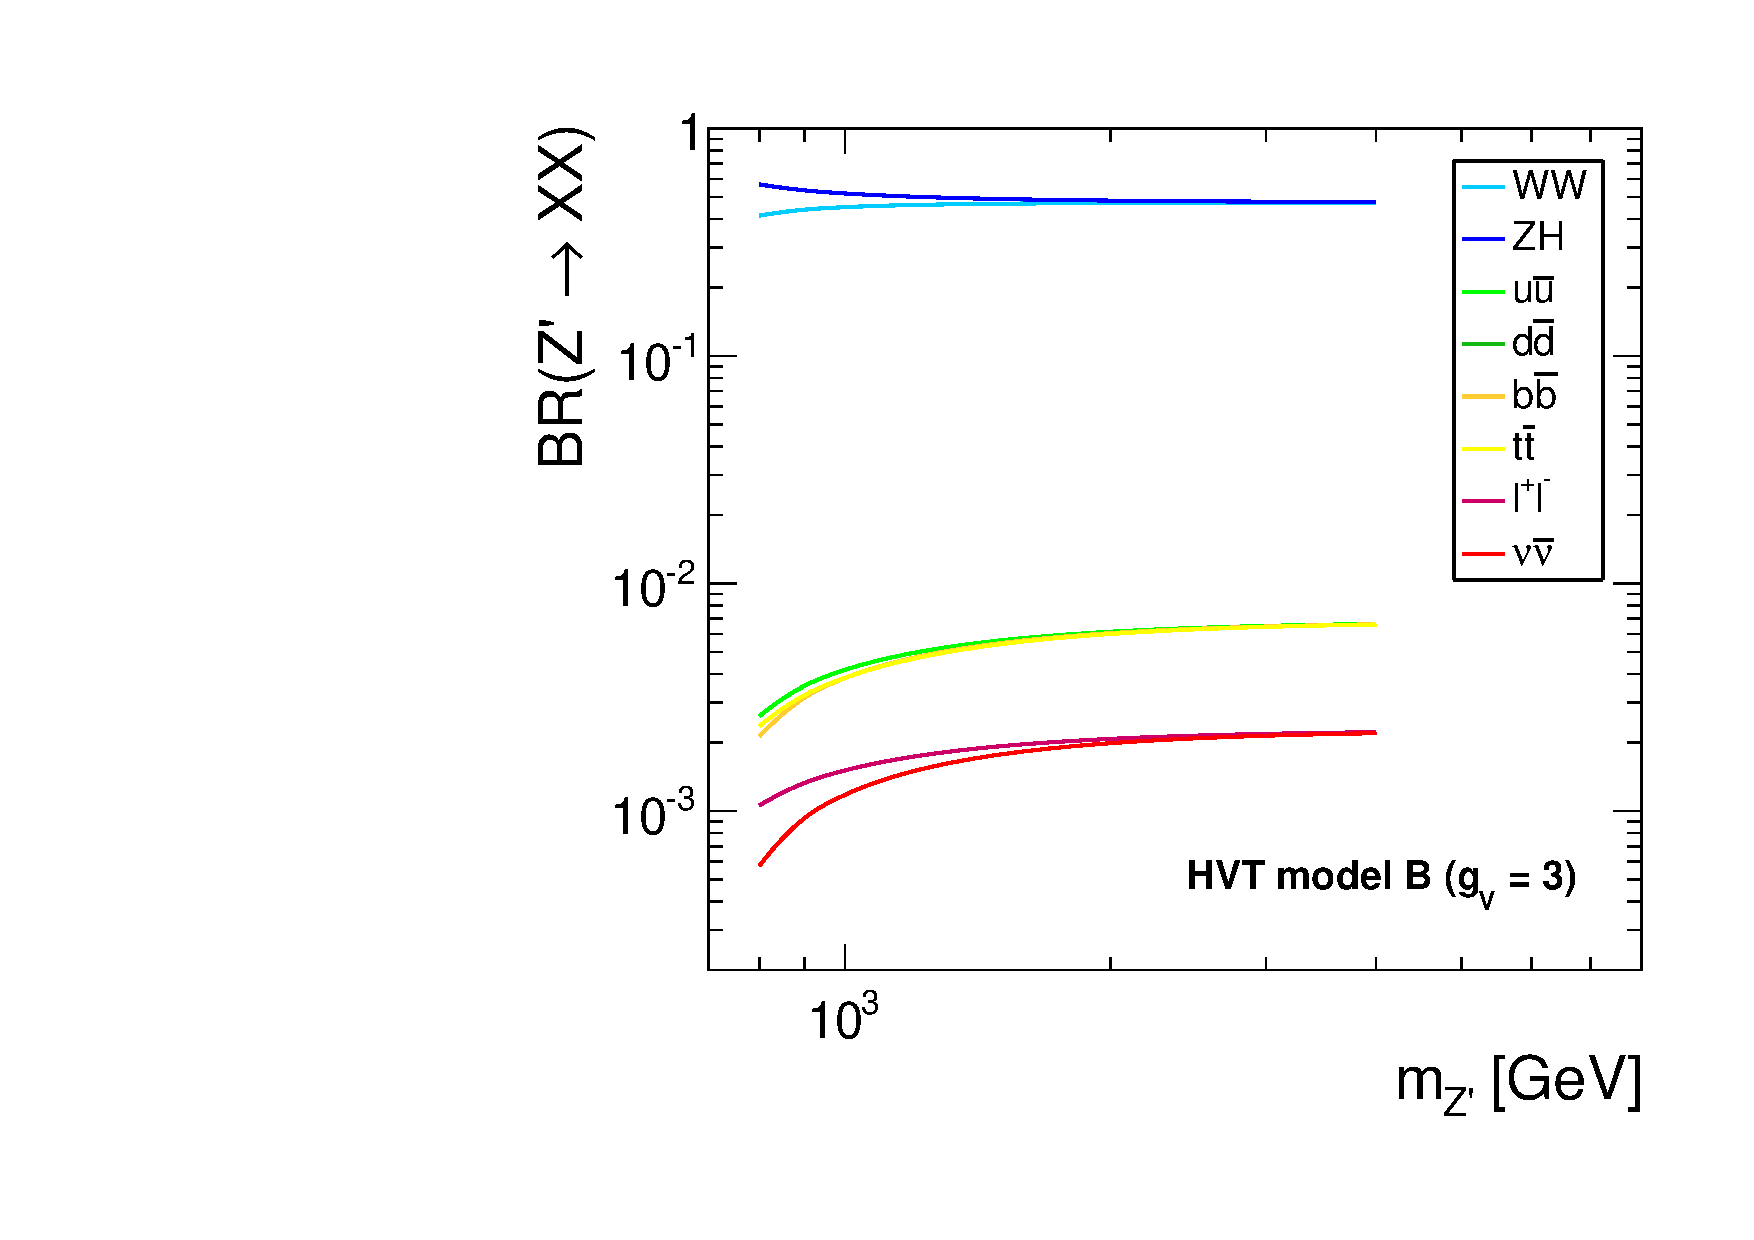
\includegraphics[width=0.45\textwidth]{\chtwo/brs-hvt-zprime-modelB.pdf}}
\caption{Branching fractions for the different decay modes of the neutral spin-1 resonance \Zpr ($V^0$) for the benchmarks (a) $\mathrm{A}_{g_V=1}$ (a) and (b) $\mathrm{B}_{g_V=3}$, as a function of the resonance mass.}
\label{fig:hvtBR}
\end{figure}

It has to be noted that the predictions of this simplified model are only valid for sufficiently narrow resonances.
In fact, several effects due to new physics, not included in this simplified framework, might contribute to the tail and radically change its prediction.
As a consequence, the results of an experimental search which is sensitive to the tail cannot be easily translated into bounds on the phenomenological parameter space.